% Created by tikzDevice version 0.12.3.1 on 2022-08-25 11:16:46
% !TEX encoding = UTF-8 Unicode
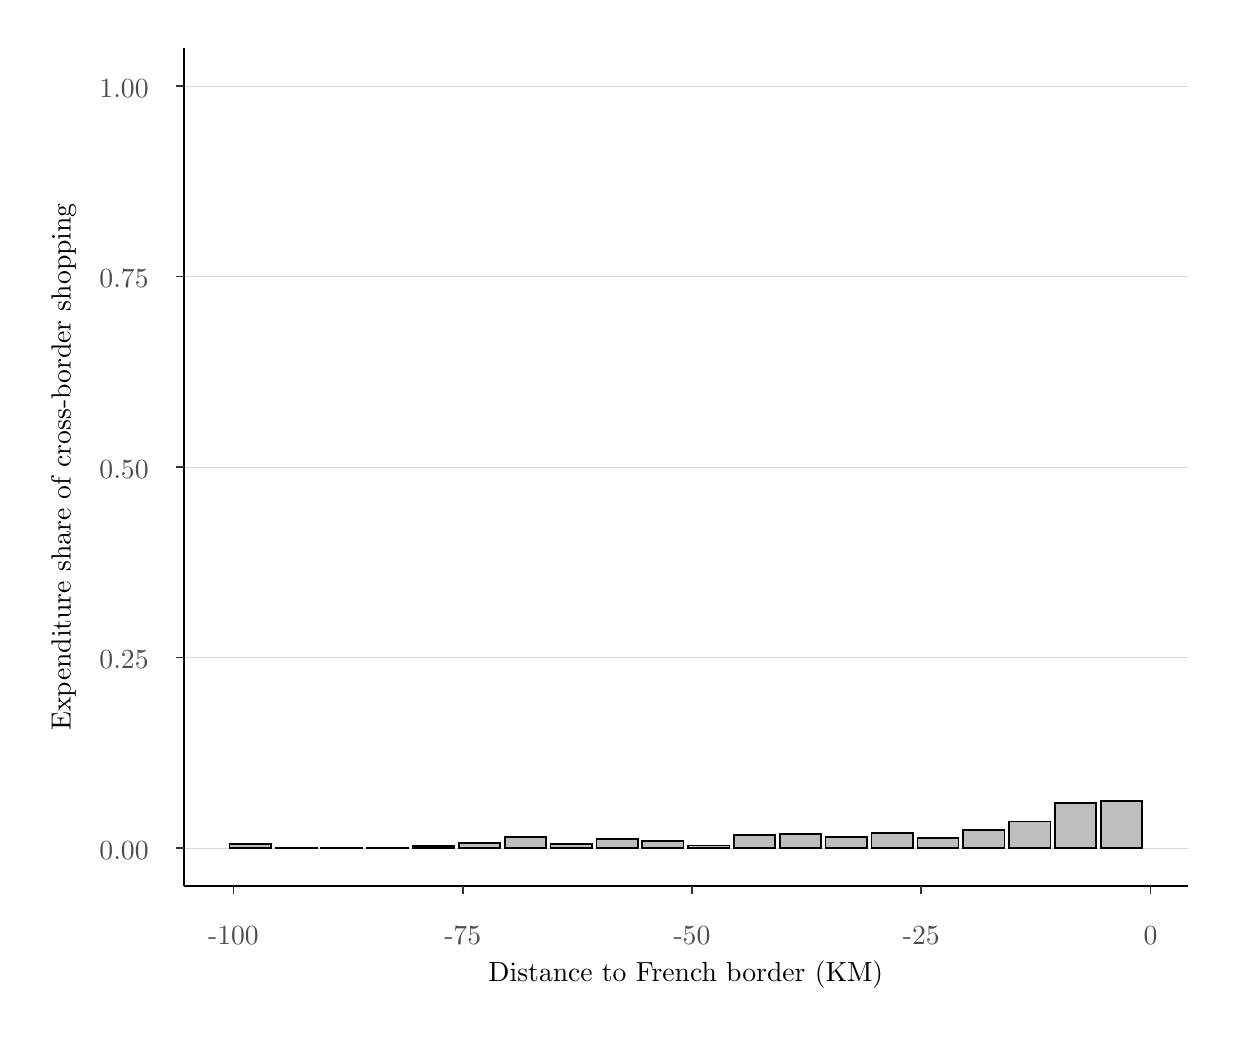
\begin{tikzpicture}[x=1pt,y=1pt]
\definecolor{fillColor}{RGB}{255,255,255}
\path[use as bounding box,fill=fillColor,fill opacity=0.00] (0,0) rectangle (433.62,361.35);
\begin{scope}
\path[clip] (  0.00,  0.00) rectangle (433.62,361.35);
\definecolor{drawColor}{RGB}{255,255,255}
\definecolor{fillColor}{RGB}{255,255,255}

\path[draw=drawColor,line width= 0.6pt,line join=round,line cap=round,fill=fillColor] ( -0.00,  0.00) rectangle (433.62,361.35);
\end{scope}
\begin{scope}
\path[clip] ( 56.47, 51.15) rectangle (419.17,354.12);
\definecolor{drawColor}{RGB}{255,255,255}

\path[draw=drawColor,line width= 0.3pt,line join=round] ( 56.47, 99.35) --
	(419.17, 99.35);

\path[draw=drawColor,line width= 0.3pt,line join=round] ( 56.47,168.21) --
	(419.17,168.21);

\path[draw=drawColor,line width= 0.3pt,line join=round] ( 56.47,237.07) --
	(419.17,237.07);

\path[draw=drawColor,line width= 0.3pt,line join=round] ( 56.47,305.92) --
	(419.17,305.92);

\path[draw=drawColor,line width= 0.3pt,line join=round] (115.77, 51.15) --
	(115.77,354.12);

\path[draw=drawColor,line width= 0.3pt,line join=round] (198.62, 51.15) --
	(198.62,354.12);

\path[draw=drawColor,line width= 0.3pt,line join=round] (281.46, 51.15) --
	(281.46,354.12);

\path[draw=drawColor,line width= 0.3pt,line join=round] (364.31, 51.15) --
	(364.31,354.12);
\definecolor{drawColor}{gray}{0.85}

\path[draw=drawColor,line width= 0.1pt,line join=round] ( 56.47, 64.92) --
	(419.17, 64.92);

\path[draw=drawColor,line width= 0.1pt,line join=round] ( 56.47,133.78) --
	(419.17,133.78);

\path[draw=drawColor,line width= 0.1pt,line join=round] ( 56.47,202.64) --
	(419.17,202.64);

\path[draw=drawColor,line width= 0.1pt,line join=round] ( 56.47,271.49) --
	(419.17,271.49);

\path[draw=drawColor,line width= 0.1pt,line join=round] ( 56.47,340.35) --
	(419.17,340.35);
\definecolor{drawColor}{RGB}{0,0,0}
\definecolor{fillColor}{gray}{0.74}

\path[draw=drawColor,line width= 0.6pt,line cap=rect,fill=fillColor] ( 72.95, 64.92) rectangle ( 87.86, 66.43);

\path[draw=drawColor,line width= 0.6pt,line cap=rect,fill=fillColor] ( 89.52, 64.92) rectangle (104.43, 64.97);

\path[draw=drawColor,line width= 0.6pt,line cap=rect,fill=fillColor] (106.09, 64.92) rectangle (121.00, 64.95);

\path[draw=drawColor,line width= 0.6pt,line cap=rect,fill=fillColor] (122.66, 64.92) rectangle (137.57, 65.12);

\path[draw=drawColor,line width= 0.6pt,line cap=rect,fill=fillColor] (139.23, 64.92) rectangle (154.14, 65.60);

\path[draw=drawColor,line width= 0.6pt,line cap=rect,fill=fillColor] (155.80, 64.92) rectangle (170.71, 66.77);

\path[draw=drawColor,line width= 0.6pt,line cap=rect,fill=fillColor] (172.37, 64.92) rectangle (187.28, 68.92);

\path[draw=drawColor,line width= 0.6pt,line cap=rect,fill=fillColor] (188.94, 64.92) rectangle (203.85, 66.44);

\path[draw=drawColor,line width= 0.6pt,line cap=rect,fill=fillColor] (205.51, 64.92) rectangle (220.42, 68.18);

\path[draw=drawColor,line width= 0.6pt,line cap=rect,fill=fillColor] (222.08, 64.92) rectangle (236.99, 67.35);

\path[draw=drawColor,line width= 0.6pt,line cap=rect,fill=fillColor] (238.64, 64.92) rectangle (253.56, 65.88);

\path[draw=drawColor,line width= 0.6pt,line cap=rect,fill=fillColor] (255.21, 64.92) rectangle (270.13, 69.59);

\path[draw=drawColor,line width= 0.6pt,line cap=rect,fill=fillColor] (271.78, 64.92) rectangle (286.70, 69.87);

\path[draw=drawColor,line width= 0.6pt,line cap=rect,fill=fillColor] (288.35, 64.92) rectangle (303.26, 68.93);

\path[draw=drawColor,line width= 0.6pt,line cap=rect,fill=fillColor] (304.92, 64.92) rectangle (319.83, 70.37);

\path[draw=drawColor,line width= 0.6pt,line cap=rect,fill=fillColor] (321.49, 64.92) rectangle (336.40, 68.51);

\path[draw=drawColor,line width= 0.6pt,line cap=rect,fill=fillColor] (338.06, 64.92) rectangle (352.97, 71.33);

\path[draw=drawColor,line width= 0.6pt,line cap=rect,fill=fillColor] (354.63, 64.92) rectangle (369.54, 74.49);

\path[draw=drawColor,line width= 0.6pt,line cap=rect,fill=fillColor] (371.20, 64.92) rectangle (386.11, 81.26);

\path[draw=drawColor,line width= 0.6pt,line cap=rect,fill=fillColor] (387.77, 64.92) rectangle (402.68, 81.95);
\end{scope}
\begin{scope}
\path[clip] (  0.00,  0.00) rectangle (433.62,361.35);
\definecolor{drawColor}{RGB}{0,0,0}

\path[draw=drawColor,line width= 0.6pt,line join=round] ( 56.47, 51.15) --
	( 56.47,354.12);
\end{scope}
\begin{scope}
\path[clip] (  0.00,  0.00) rectangle (433.62,361.35);
\definecolor{drawColor}{gray}{0.30}

\node[text=drawColor,anchor=base east,inner sep=0pt, outer sep=0pt, scale=  1.00] at ( 43.72, 60.79) {0.00};

\node[text=drawColor,anchor=base east,inner sep=0pt, outer sep=0pt, scale=  1.00] at ( 43.72,129.65) {0.25};

\node[text=drawColor,anchor=base east,inner sep=0pt, outer sep=0pt, scale=  1.00] at ( 43.72,198.51) {0.50};

\node[text=drawColor,anchor=base east,inner sep=0pt, outer sep=0pt, scale=  1.00] at ( 43.72,267.36) {0.75};

\node[text=drawColor,anchor=base east,inner sep=0pt, outer sep=0pt, scale=  1.00] at ( 43.72,336.22) {1.00};
\end{scope}
\begin{scope}
\path[clip] (  0.00,  0.00) rectangle (433.62,361.35);
\definecolor{drawColor}{gray}{0.20}

\path[draw=drawColor,line width= 0.6pt,line join=round] ( 53.72, 64.92) --
	( 56.47, 64.92);

\path[draw=drawColor,line width= 0.6pt,line join=round] ( 53.72,133.78) --
	( 56.47,133.78);

\path[draw=drawColor,line width= 0.6pt,line join=round] ( 53.72,202.64) --
	( 56.47,202.64);

\path[draw=drawColor,line width= 0.6pt,line join=round] ( 53.72,271.49) --
	( 56.47,271.49);

\path[draw=drawColor,line width= 0.6pt,line join=round] ( 53.72,340.35) --
	( 56.47,340.35);
\end{scope}
\begin{scope}
\path[clip] (  0.00,  0.00) rectangle (433.62,361.35);
\definecolor{drawColor}{RGB}{0,0,0}

\path[draw=drawColor,line width= 0.6pt,line join=round] ( 56.47, 51.15) --
	(419.17, 51.15);
\end{scope}
\begin{scope}
\path[clip] (  0.00,  0.00) rectangle (433.62,361.35);
\definecolor{drawColor}{gray}{0.20}

\path[draw=drawColor,line width= 0.6pt,line join=round] ( 74.35, 48.40) --
	( 74.35, 51.15);

\path[draw=drawColor,line width= 0.6pt,line join=round] (157.20, 48.40) --
	(157.20, 51.15);

\path[draw=drawColor,line width= 0.6pt,line join=round] (240.04, 48.40) --
	(240.04, 51.15);

\path[draw=drawColor,line width= 0.6pt,line join=round] (322.89, 48.40) --
	(322.89, 51.15);

\path[draw=drawColor,line width= 0.6pt,line join=round] (405.73, 48.40) --
	(405.73, 51.15);
\end{scope}
\begin{scope}
\path[clip] (  0.00,  0.00) rectangle (433.62,361.35);
\definecolor{drawColor}{gray}{0.30}

\node[text=drawColor,anchor=base,inner sep=0pt, outer sep=0pt, scale=  1.00] at ( 74.35, 30.14) {-100};

\node[text=drawColor,anchor=base,inner sep=0pt, outer sep=0pt, scale=  1.00] at (157.20, 30.14) {-75};

\node[text=drawColor,anchor=base,inner sep=0pt, outer sep=0pt, scale=  1.00] at (240.04, 30.14) {-50};

\node[text=drawColor,anchor=base,inner sep=0pt, outer sep=0pt, scale=  1.00] at (322.89, 30.14) {-25};

\node[text=drawColor,anchor=base,inner sep=0pt, outer sep=0pt, scale=  1.00] at (405.73, 30.14) {0};
\end{scope}
\begin{scope}
\path[clip] (  0.00,  0.00) rectangle (433.62,361.35);
\definecolor{drawColor}{RGB}{0,0,0}

\node[text=drawColor,anchor=base,inner sep=0pt, outer sep=0pt, scale=  1.00] at (237.82, 16.79) {Distance to French border (KM)};
\end{scope}
\begin{scope}
\path[clip] (  0.00,  0.00) rectangle (433.62,361.35);
\definecolor{drawColor}{RGB}{0,0,0}

\node[text=drawColor,rotate= 90.00,anchor=base,inner sep=0pt, outer sep=0pt, scale=  1.00] at ( 15.49,202.64) {Expenditure share of cross-border shopping};
\end{scope}
\end{tikzpicture}
